\documentclass[12pt]{article}
\usepackage[utf8]{inputenc}
\usepackage[left=2cm,right=2cm,top=2cm,bottom=2cm]{geometry}
\usepackage{graphicx, amsmath}
\usepackage[small]{caption}
\usepackage{subcaption}
\usepackage{url}
\setlength{\parskip}{\baselineskip}
\graphicspath{ {images/} }

\usepackage{hyperref}
\hypersetup{
	colorlinks=true,
	linkcolor=blue,     
	urlcolor=blue,
	citecolor=blue,
}


\begin{document}

	\thispagestyle{empty}

	\begin{center}
		{\Large \bf Expected value and variance}\\
		Gabriela S\'anchez Y.\\
		5064
	\end{center}
  
	In this activity a serie of exercises of the book Introducción to Probability \cite{prob2003} are solved.
	
	{\bf Exercise 1, page 247}
	
	{\em A card is drawn at random from a deck consisting of cards numbered $2$ through $10$. A player wins $1$ dollar if the number on the card is odd and loses $1$ dollar if the number if even. What is the expected value of his winnings?}
	
	Let $X$ be the card selected and $\phi(X)$ define as in equation (\ref{odd-even}). 
	\begin{equation}
	\phi(X)= \left\{ \begin{array}{rc}
	1, & x \,\, \text{is odd},	\\
	-1, & x \,\, \text{is even}. 
	\end{array}
	\right.
	\label{odd-even}
	\end{equation}
	
	The sample space of $X$ is the set $\{2, 3, \ldots, 10\}$ and $P(X=2) = \cdots = P(X=10) = \frac{1}{9}$. Therefore
	\begin{eqnarray*}
	E[\phi(X)] &=& \sum_{x \in \Omega} \phi(x) \cdot P(X=x) \\
	&=& -1 \cdot \left(\frac{1}{9} \right) + 1 \cdot \left( \frac{1}{9} \right) -1 \cdot \left(\frac{1}{9} \right) + \ldots -1 \cdot \left(\frac{1}{9} \right) \\
	&=& -1 \cdot \left(\frac{5}{9} \right) + 1 \cdot \left( \frac{4}{9} \right) \\
	&=& -\frac{1}{9}.
	\end{eqnarray*}
	
	{\bf Excercise 6, page 247}
	
	{\em A die is rolled twice. Let $X$ denote the sum of the two numbers that turn up, and Y the difference of the numbers (specifically, the number on the first roll minus the number on the second). Show that $E[XY] = E[X]E[Y]$. Are $X$ and $Y$ independent?}
	
	Let $D_1$ and $D_2$ the outcomes on the first and second roll, respectively. Then $X = D_1 + D_2$ and $Y=D_1 - D_2$. 
	
	$D_1$ and $D_2$ have the same outcomes with the same probabilities so it is clear that $E[D_1] = E[D_2]$. Therefore,
	\begin{eqnarray*}
	E[XY] &=& E[(D_1 + D_2)\cdot(D_1 - D_2)] \\
	&=& E[(D_1)^2 - (D_2)^2] \\
	&=& E[(D_1)^2] - E[(D_2)^2] = 0,
	\end{eqnarray*}
	and $E[Y] = E[D_1] - E[D_2] = 0$. Then $E[X]E[Y] = 0$, and $E[XY] = E[X]E[Y]$.
	 
	Even though $E[XY] = E[X]E[Y]$, $X$ and $Y$ are not independent. Two ramdom variables are independent if equation (\ref{independent}) is satisfied for any $x \in X$ and $y \in Y$.
	\begin{equation}
	P(X = x, Y = y) = P(X=x) P(Y=y).
	\label{independent}
	\end{equation}
	
	The possible outcomes of the rolles are
	\begin{center}
		\begin{tabular}{cccccc}
		(1,1) & (1,2) & (1,3) & (1,4) & (1,5) & (1,6) \\
		(2,1) & (2,2) & (2,3) & (2,4) & (2,5) & (2,6) \\
		(3,1) & (3,2) & (3,3) & (3,4) & (3,5) & (3,6) \\
		(4,1) & (4,2) & (4,3) & (4,4) & (4,5) & (4,6) \\
		(5,1) & (5,2) & (5,3) & (5,4) & (5,5) & (5,6) \\
		(6,1) & (6,2) & (6,3) & (6,4) & (6,5) & (6,6) \\	
		\end{tabular}
	\end{center}
	each one with probability of 1/36. 
	
	Note that $P(X=6, Y=0) = 1/36$ because this can only happend when $D_1 = 3$ and $D_2 = 3$, and  
	\begin{equation*}
	P(X=6)P(Y=0) = \frac{5}{36} \cdot \frac{6}{36} = \frac{5}{36} \cdot \frac{1}{6} = \frac{5}{216}.
	\end{equation*}
	
	Therefore $P(X = x, Y = y) \neq P(X=x) P(Y=y)$ for $x=6$ and $y= 0$, so it has been proven that $X$ and $Y$ are not independent.
	
	{\bf Exercise 15, page 249}
	
	{\em A box contains two gold balls and three silver balls. You are allowed to choose successively balls from the box at random. You win 1 dollar each time you draw a gold ball and lose 1 dollar each time you draw a silver ball. After a draw, the ball is not replaced. Show that, if you draw until you are ahead by 1 dollar or until there are no more gold balls, this is a favorable game.}
	
	The possible outcomes of the draw when the player is ahead by 1 dollar or until there are no more gold balls is shown in Table \ref{table_outcomes}, where $S$ and $G$ represents an outcome of a silver and gold ball, respectively.
	\begin{table}
		\caption{Possible outcomes.}
		\label{table_outcomes}
		\centering
		\begin{tabular}{lcc}
			\hline
			\bf Outcome & \bf Probability & \bf Winnings \\
			\hline
			\vspace{0.2cm}
			G & $\frac{2}{5}$ & 1 \\
			\vspace{0.2cm}
			SGG & $\frac{3}{5} \cdot \frac{2}{4} \cdot \frac{1}{3} = \frac{1}{10}$ & 1 \\
			\vspace{0.2cm}
			GSG & $\frac{2}{5} \cdot \frac{3}{4} \cdot \frac{1}{3} = \frac{1}{10}$ & 1 \\
			\vspace{0.2cm}
			GG & $\frac{2}{5} \cdot \frac{1}{4} = \frac{1}{10}$ & 2 \\
			\vspace{0.2cm}
			SGSG & $\frac{3}{5} \cdot \frac{2}{4} \cdot \frac{2}{3} \cdot \frac{1}{2} = \frac{1}{10}$ & 0 \\
			\vspace{0.2cm}
			SSGG & $\frac{3}{5} \cdot \frac{2}{4} \cdot \frac{2}{3} \cdot \frac{1}{2} = \frac{1}{10}$ & 0 \\
			\vspace{0.2cm}
			SSGSG & $\frac{3}{5} \cdot \frac{2}{4} \cdot \frac{2}{3} \cdot \frac{1}{2} \cdot 1 = \frac{1}{10}$ & -1 \\
			\vspace{0.2cm}
			SGSSG & $\frac{3}{5} \cdot \frac{2}{4} \cdot \frac{2}{3} \cdot \frac{1}{2} \cdot 1 = \frac{1}{10}$ & -1 \\
			\vspace{0.2cm}
			SSSGG & $\frac{3}{5} \cdot \frac{2}{4} \cdot \frac{1}{3} \cdot 1 \cdot 1 = \frac{1}{10}$ & -1 \\
			\hline
		\end{tabular}
	\end{table}

	Then 
	\begin{eqnarray*}
	E[X] &=& 1 \cdot \frac{2}{5} + 1 \cdot \frac{1}{10} + 1 \cdot \frac{1}{10} + 2 \cdot \frac{1}{10} + 0 \cdot \frac{1}{10} + 0 \cdot \frac{1}{10} - 1 \cdot \frac{1}{10} - 1 \cdot \frac{1}{10} - 1\cdot \frac{1}{10} \\
	&=& \frac{2}{5} + \frac{2}{10} + \frac{2}{10} - \frac{3}{10} \\
	&=& \frac{2}{5} + \frac{4}{10} - \frac{3}{10} \\
	&=& \frac{2}{5} + \frac{1}{10} = \frac{1}{2}.
	\end{eqnarray*}

	Given that $E[X] > 0$, playing until the ahead by 1 dollar is kept or until there are no more gold balls, the game will be favorable. 
	
	{\bf Exercise 18, page 249}
	
	{\em Exactly one of six similar keys opens a certain door. If you try the keys, one after another, what is the expected number of keys that you will have to try before success?}
	
	It is assumed that once a key is tried it is discarted. Let $X$ be the number of failures before success. Having two failures before success means that the sequence of tried keys was $FFS$, where $F$ represents a failure and $S$ a success. The probability of this sequence (i.e., having two failures before success) can be calculated using the tree in Figure \ref{keys}, so $P(X=2) = \frac{5}{6} \cdot \frac{4}{5} \cdot \frac{1}{4} = \frac{1}{6}$. 
	
	The possible values of $X$ are $\{0, 1, \ldots, 5\}$ and $P(X = 0) = P(X = 1) = \ldots = P(X = 5) = \frac{1}{6}$ (see Figure \ref{keys}). Thus
	\begin{eqnarray*}
	E[X] &=& 0 \cdot \frac{1}{6} + 1 \cdot \frac{1}{6} + 2 \cdot \frac{1}{6} + 3 \cdot \frac{1}{6} + 4 \cdot \frac{1}{6} + 5 \cdot \frac{1}{6} \\
	&=& \frac{15}{6} = \frac{5}{2}.
	\end{eqnarray*}

	\begin{figure}
	\centering
	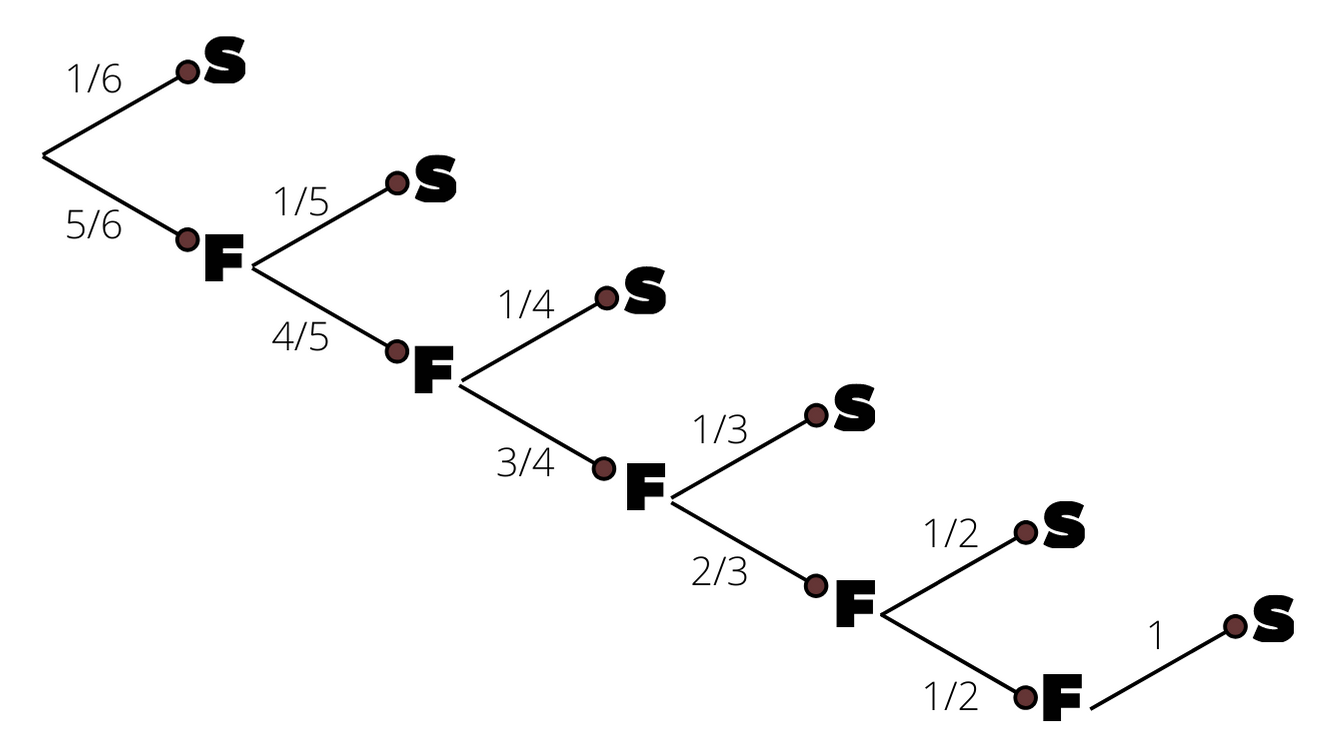
\includegraphics[scale=0.2]{exercise_keys.png}	
	\caption{Tree for excercise 18, page 249.}
	\label{keys}
	\end{figure}
	
	{\bf Exercise 19, page 249}
	
	{\em A multiple choice exam is given. A problem has four possible answers, and exactly one answer is correct. The student is allowed to choose a subset of the four possible answers as his answer. If his chosen subset contains the correct answer, the student receives three points, but he loses one point for each wrong answer in his chosen subset. Show that if he just guesses a subset uniformly and randomly his expected score is zero.}
	
	It does not make any sense that the student do not choose a subset, so he can choose subsets of one, two, three or four possible answers.
	
	Let $R_1, R_2, R_3, R_4$ the four possible answers and without loss of generality let $R_1$ be the right one.
	
	\begin{itemize}
		\item Subsets of one answer
	\end{itemize}
	
	In this scenario are four options $\{R_1\}, \{R_2\}, \{R_3\}$ and $\{R_4\}$ each one of them with a probability of been choose equal to $\frac{1}{4}$. Then the espected value is
	\begin{equation*}
	3 \left( \frac{1}{4} \right) - 1 \left( \frac{1}{4}\right) - 1 \left(\frac{1}{4}\right) - 1 \left( \frac{1}{4}\right) = 0.
	\end{equation*}  
	
	\begin{itemize}
		\item Subsets of two answers
	\end{itemize}
	
	The number of possible subsets with two answers are $\binom{4}{2} = 6$: $\{R_1, R_2\}, \{R_1, R_3\}$, $\{R_1, R_4\}$, $\{R_2, R_3\}$, $\{R_2, R_4\}$ and $\{R_3, R_4\}$. The right answer $R_1$ is in three of these subsets. The espected value in this scenario is
	\begin{equation*}
	3 \left(\frac{3}{6}\right) - 1 \left(\frac{3}{6}\right) - 2 \left(\frac{1}{6}\right) - 2 \left(\frac{1}{6}\right) - 2 \left(\frac{1}{6}\right) = 0.
	\end{equation*}
	
	\begin{itemize}
		\item Subsets of three answers
	\end{itemize}
	In this case the possible subsets are $\binom{4}{3} = 4$: $\{R_1, R_2, R_3\}, \{R_1, R_3, R_4\}$, $\{R_2, R_3, R_4\}$ and $\{R_1, R_2, R_4\}$. Again, the right answer is in three of these subsets. The espected value is
	\begin{equation*}
	3 \left(\frac{3}{4}\right) - 2 \left(\frac{3}{4}\right) - 3 \left(\frac{1}{4}\right) = 0.
	\end{equation*} 
	
	\begin{itemize}
		\item Subsets of four answers
	\end{itemize}
	
	There is only one possible subset $\{R_1, R_2, R_3, R_4\}$. The espected value is
	\begin{equation*}
	3 \cdot (1) - 3 \cdot (1) = 0.
	\end{equation*}
	
	
	{\bf Exercise 1, page 263}
	
	{\em A number is chosen at random from the set $S = \lbrace -1, 0, 1 \rbrace$. Let $X$ be the number chosen. Find the expected value, variance, and standard deviation of $X$.}
	
	\begin{equation*}
	E[X] = -1 \cdot \frac{1}{3} + 0 \cdot \frac{1}{3} + 1 \cdot \frac{1}{3} = 0.
	\end{equation*}
	
	Recalling that $V[X] = E[X^2] - \mu^2$, where $\mu = E[X]$, then
	\begin{equation*}
	V[X] = E[X^2] - (0)^2 = (-1)^2 \cdot \frac{1}{3} + (0)^2 \cdot \frac{1}{3} + (1)^2 \cdot \frac{1}{3} = \frac{2}{3},
	\end{equation*}
	and $D[X] = \sqrt{V[X]} = \sqrt{\frac{2}{3}}$.
	
	
	{\bf Exercise 9, page 264}
	
	{\em A die is loaded so that the probability of a face coming up is proportional to the number on that face. The die is rolled with outcome $X$. Find $V(X)$ and $D(X)$.}
	
	Let $X$ be the outcome of the die, then $P(X = x) = x\cdot p$. Recall that $\displaystyle\sum_{i=1}^{6} i\cdot p = 1$, therefore $p = \frac{1}{21}$. 
	
	To find $V[X]$ it is necessary to find $E[X]$ and $E[X^2]$ first, so 
	\begin{eqnarray*}
	E[X] &=& 1 \cdot p + 2 \cdot 2p + 3 \cdot 3p + 4 \cdot 4p + 5 \cdot 5p + 6 \cdot 6p \\
	&=& p (1 + 4 + 9 + 16 + 25 + 36) \\
	&=& 91p \\
	&=& \frac{91}{21},
	\end{eqnarray*}
	and 
	\begin{eqnarray*}
	E[X^2] &=& \sum_{i=1}^{6} i^2 \cdot (i\cdot p) \\
	&=& p \sum_{i=1}^{6} i^3 \\
	&=& p \left( \frac{ 6^2 \cdot 7^2}{4} \right) \\
	&=& p \cdot \frac{1764}{4} \\
	&=& \frac{441}{21} = 21.
	\end{eqnarray*}
	
	Then 
	\begin{eqnarray*}
	V[X] &=& E[X^2] - \left(E[X]\right)^2 \\
	&=& 21 - \left( \frac{91}{21} \right)^2 \\
	&=& \frac{20}{9}, 
	\end{eqnarray*}
	and $D[X] = \sqrt{V[X]} = \sqrt{\frac{20}{9}} = \frac{2}{3} \sqrt{5}$.
	
	{\bf Exercise 12, page 264}
	
	{\em Let $X$ be a random variable with $\mu = E(X)$ and $\sigma^2 = V(X)$. Define $X^* = (X-\mu)/\sigma$. The random variable $X^*$ is called the \textit{standardized random variable} associated with $X$. Show that this standardized random variable has expected value 0 and variance 1.}
	
	Bearing in mind the properties of linearity of the expected value, the following is obtained 
	\begin{eqnarray*}
	E[X^*] &=& E \left[ \frac{X - \mu }{\sigma}\right]\\
	 &=& E \left[ \frac{1}{\sigma}\left( X - \mu \right)\right] \\
	 &=& \frac{1}{\sigma} \cdot E[X - \mu] \\
	&=& \frac{1}{\sigma} \cdot \left( E[X] - E[\mu] \right) \\
	&=& \frac{1}{\sigma} \cdot \left( \mu - \mu \right) = 0,
	\end{eqnarray*}
	and 
	\begin{eqnarray*}
	V[X^*] &=& E[(X^* - 0)^2] \\
	&=& E\left[\left(\frac{X - \mu}{\sigma} \right)^2 \right] \\
	&=& E\left[\frac{1}{\sigma^2} \cdot (X - \mu)^2 \right] \\
	&=& \frac{1}{\sigma^2} \cdot E[(X - \mu)^2] \\
	&=& \frac{1}{\sigma^2} \cdot V[X] \\
	&=& \frac{1}{\sigma^2} \cdot \sigma^2 = 1.
	\end{eqnarray*}
	
	{\bf Exercise 3, page 278}
	
	{\em The lifetime, measure in hours, of the ACME super light bulb is a random variable T with density function \(f_T (t) = \lambda^2 te^{- \lambda t}\), where \(\lambda = 0.05\). What is the expected lifetime of this light bulb? What is its variance?}
	
	The expected lifetime of the light bulb is given by the integral in equation (\ref{ev_bulb})
	\begin{equation}
	E[T] = \int_{0}^{\infty} t \cdot \left( \lambda^2 t e^{-\lambda t} \right) \, dt.
	\label{ev_bulb}
	\end{equation}
	
	One can rewrite integral in equation (\ref{ev_bulb}) as follows
	\begin{equation}
	E[T] = \lambda^2 \int_{0}^{\infty}  t^2 e^{-\lambda t} \, dt.
	\label{ev_bulb_rewrite}
	\end{equation}
	
	To compute the expected lifetime of the light bulb, first the integral 
	\begin{equation*}
	\int t^2 e^{-\lambda t} \, dt
	\end{equation*}
	is solved integrating by parts. Thus
	\begin{equation}
	\int t^2 \, e^{-\lambda t} dt = -\frac{t^2}{\lambda} e^{-\lambda t} + \frac{2}{\lambda} \int te^{-\lambda t} \, dt.
	\label{integral_bulb}
	\end{equation}
	The integral $\int te^{-\lambda t} dt$ is solved using integration by parts again
	\begin{equation*}
	\int te^{-\lambda t} dt = - \frac{t}{\lambda} e^{-\lambda t} + \frac{1}{\lambda} \int e^{-\lambda t} \, dt.
	\end{equation*}
	The last integral can be solve directly by formulas, then
	\begin{equation}
	\int te^{-\lambda t} dt = - \frac{t}{\lambda} e^{-\lambda t} - \frac{1}{\lambda^2} e^{-\lambda t}.
	\label{integral_bulb_parts}
	\end{equation}
	The result found in (\ref{integral_bulb_parts}) is replaced into equation (\ref{integral_bulb}), so
	\begin{eqnarray}
	\int t^2 \, e^{-\lambda t} dt &=& -\frac{t^2}{\lambda} e^{-\lambda t} + \frac{2}{\lambda} \left(  - \frac{t}{\lambda} e^{-\lambda t} - \frac{1}{\lambda^2} e^{-\lambda t} \right) \nonumber \\
	&=& -\frac{t^2}{\lambda} e^{-\lambda t} - \frac{2t}{\lambda^2} e^{-\lambda t} - \frac{2}{\lambda^3} e^{-\lambda t} \nonumber \\
	&=& -e^{-\lambda t} \left( \frac{\lambda^2 t^2 + 2\lambda t + 2}{\lambda^3} \right) \label{result_integral_bulb}.
	\end{eqnarray}
	Finally the result in (\ref{result_integral_bulb}) is replaced in equation (\ref{ev_bulb_rewrite}) 
	\begin{eqnarray*}
	E[T] &=& \lambda^2 \left. \left[ -e^{-\lambda t} \left( \frac{\lambda^2 t^2 + 2\lambda t + 2}{\lambda^3} \right) \right] \right|_{0}^{\infty} \\
	&=& \lambda^2 \cdot \frac{2}{\lambda^3} \\
	&=& \frac{2}{\lambda}.
	\end{eqnarray*}
	
	To compute the variance it is neccesary to solve the integral in equation (\ref{integral_var})
	\begin{equation}
	\int t^2 \left( \lambda^2 t e^{-\lambda t} \right) \, dt = \lambda^2 \int t^3e^{-\lambda t} \, dt.
	\label{integral_var}
	\end{equation}
	
	The integral on the right side of equation (\ref{integral_var}) can be solved integrating by parts
	\begin{equation}
	\int t^3e^{-\lambda t} \, dt = -\frac{t^3}{\lambda}e^{-\lambda t} + \frac{3}{\lambda} \int t^2 \, e^{-\lambda t}\, dt.
	\label{integral_var2}
	\end{equation}
	Note that the integral in equation (\ref{integral_var2}) was already calculated so
	\begin{eqnarray}
	\int t^3e^{-\lambda t} \, dt &=& -\frac{t^3}{\lambda}e^{-\lambda t} + \frac{3}{\lambda} \cdot \left[- e^{-\lambda t} \left( \frac{\lambda^2 t^2 + 2\lambda t + 2}{\lambda^3} \right) \right] \nonumber \\
	&=& -\frac{t^3}{\lambda}e^{-\lambda t} - e^{-\lambda t} \left( \frac{3\lambda^2 t^2 + 6\lambda t + 6}{\lambda^4} \right) \nonumber \\
	&=& - e^{-\lambda t} \left( \frac{\lambda^3t^3 + 3\lambda^2 t^2 + 6\lambda t + 6}{\lambda^4} \right).
	\label{sol_integral_var}
	\end{eqnarray}
	
	Using the result in equation (\ref{sol_integral_var}) the variance is
	\begin{eqnarray*}
	V[T] &=& \int_{0}^{\infty} t^2 \left( \lambda^2 t e^{-\lambda t} \right) \, dt - \left(\frac{2}{\lambda}\right)^2 \\
	&=& \lambda^2 \int_{0}^{\infty} t^3e^{-\lambda t} \, dt - \frac{4}{\lambda^2} \\
	&=& \lambda^2 \left. \left[- e^{-\lambda t} \left( \frac{\lambda^3t^3 + 3\lambda^2 t^2 + 6\lambda t + 6}{\lambda^4} \right)\right] \right|_{0}^{\infty} - \frac{4}{\lambda^2} \\
	&=& \lambda^2 \cdot \frac{6}{\lambda^4} - \frac{4}{\lambda^2}\\ 
	&=& \frac{2}{\lambda^2}.
	\end{eqnarray*}

	Bearing in mind that $\lambda=0.05$ the expected lifetime of the light bulb is $E[T] = 40$ hours and its variance $V[T] = 800$ hours.
	
	{\bf Exercise 12, page 280}
	
	{\em Find $E[X^Y]$, where $X$ and $Y$ are independent random variables which are uniform on [0, 1]. Then verify your answer by simulation.}
	
	\begin{eqnarray*}
	E[X^Y] &=& \int_{0}^{1} \int_{0}^{1} x^y dx dy \\
	&=& \int_{0}^{1}  \left. \left[ \frac{x^{y+1}}{y+1} \right] \right|_{0}^{1} dy \\
	&=& \int_{0}^{1}  \left( \frac{1^{y+1}}{y+1} - \frac{0^{y+1}}{y+1} \right) dy \\
	&=& \int_{0}^{1}  \left( \frac{1}{y+1} \right) dy \\
	&=& \left. \ln (y+1) \right|_{0}^{1}\\
	&=& \ln(2) \approx 0.6931
	\end{eqnarray*}
	
\bibliographystyle{plain}
\bibliography{biblio}

\end{document}

%%@article{wu2020single,
%title={Single-cell RNA expression profiling of ACE2, the putative receptor of Wuhan 2019-nCoV, in the nasal tissue},
%author={Wu, Chao and Zheng, Shufa and Chen, Yu and Zheng, Min},
%journal={MedRxiv},
%year={2020},
%publisher={Cold Spring Harbor Laboratory Press}
%}
